%!TEX root = ../MasterThesis.tex

\chapter{Concept and Design of the System} % (fold)
\label{cha:design_system}

This main part of the Master thesis looks into a concept and design for a collaborative system that will improve the situation described in the scenario in Section~\ref{sec:scope_thesis}. Initially the chapter will discuss the overall concept of the system on an high level without going to much into implementation specifics. This will answer the question of what the system is and should be able to achieve. After this initial view on the concept of the system the chapter will further look into existing design approaches and discusses why they are of no use for this specific scenario. Lastly a novel system design approach is proposed, which is based on Semantic Web and peer-to-peer communication technologies to improve the current situation and support the investigation of E-commerce fraud incidents.

% sub chapter design overview
%!TEX root = ../MasterThesis.tex

\section{Concept of System}
\label{sec:system_concept}

Based on the explanations in Chapter~\ref{cha:context_analysis}, and especially the scope definition for this Master thesis in Section~\ref{sec:scope_thesis}, the collaborative system for investigating E-commerce fraud incidents have to answer the central question:\@

\begin{quotation}
    \textit{Is this really a fraudulent E-commerce transaction?}
\end{quotation}

The relevant stakeholders, that need to be involved in the investigation process, are:\@

\begin{enumerate}
    \item \textbf{merchant}, who can provide additional information of each E-commerce transaction in question
    \item \textbf{\gls{PSP}/issuer}, whose offer information about the credit card usage pattern and the original credit card owner
    \item \textbf{\gls{LSP}}, who can offer information about whether the order has already been shipped or not, and in the former case to whom it has been handed over
    \item \textbf{\gls{ISP}}, who can on request give hints whether a consumer has fallen victim to a phishing attack based on her Internet access logs
\end{enumerate}

Ideally each of them would make parts of their internal data structures available for the other participants to access and query for. This would allow the stakeholder, who has to authorize or validate a suspecious credit card payment, to analyse all available information, as depicted in the Figure~\ref{fig:images_system_overview}.\@

\begin{figure}[H]
	\centering
		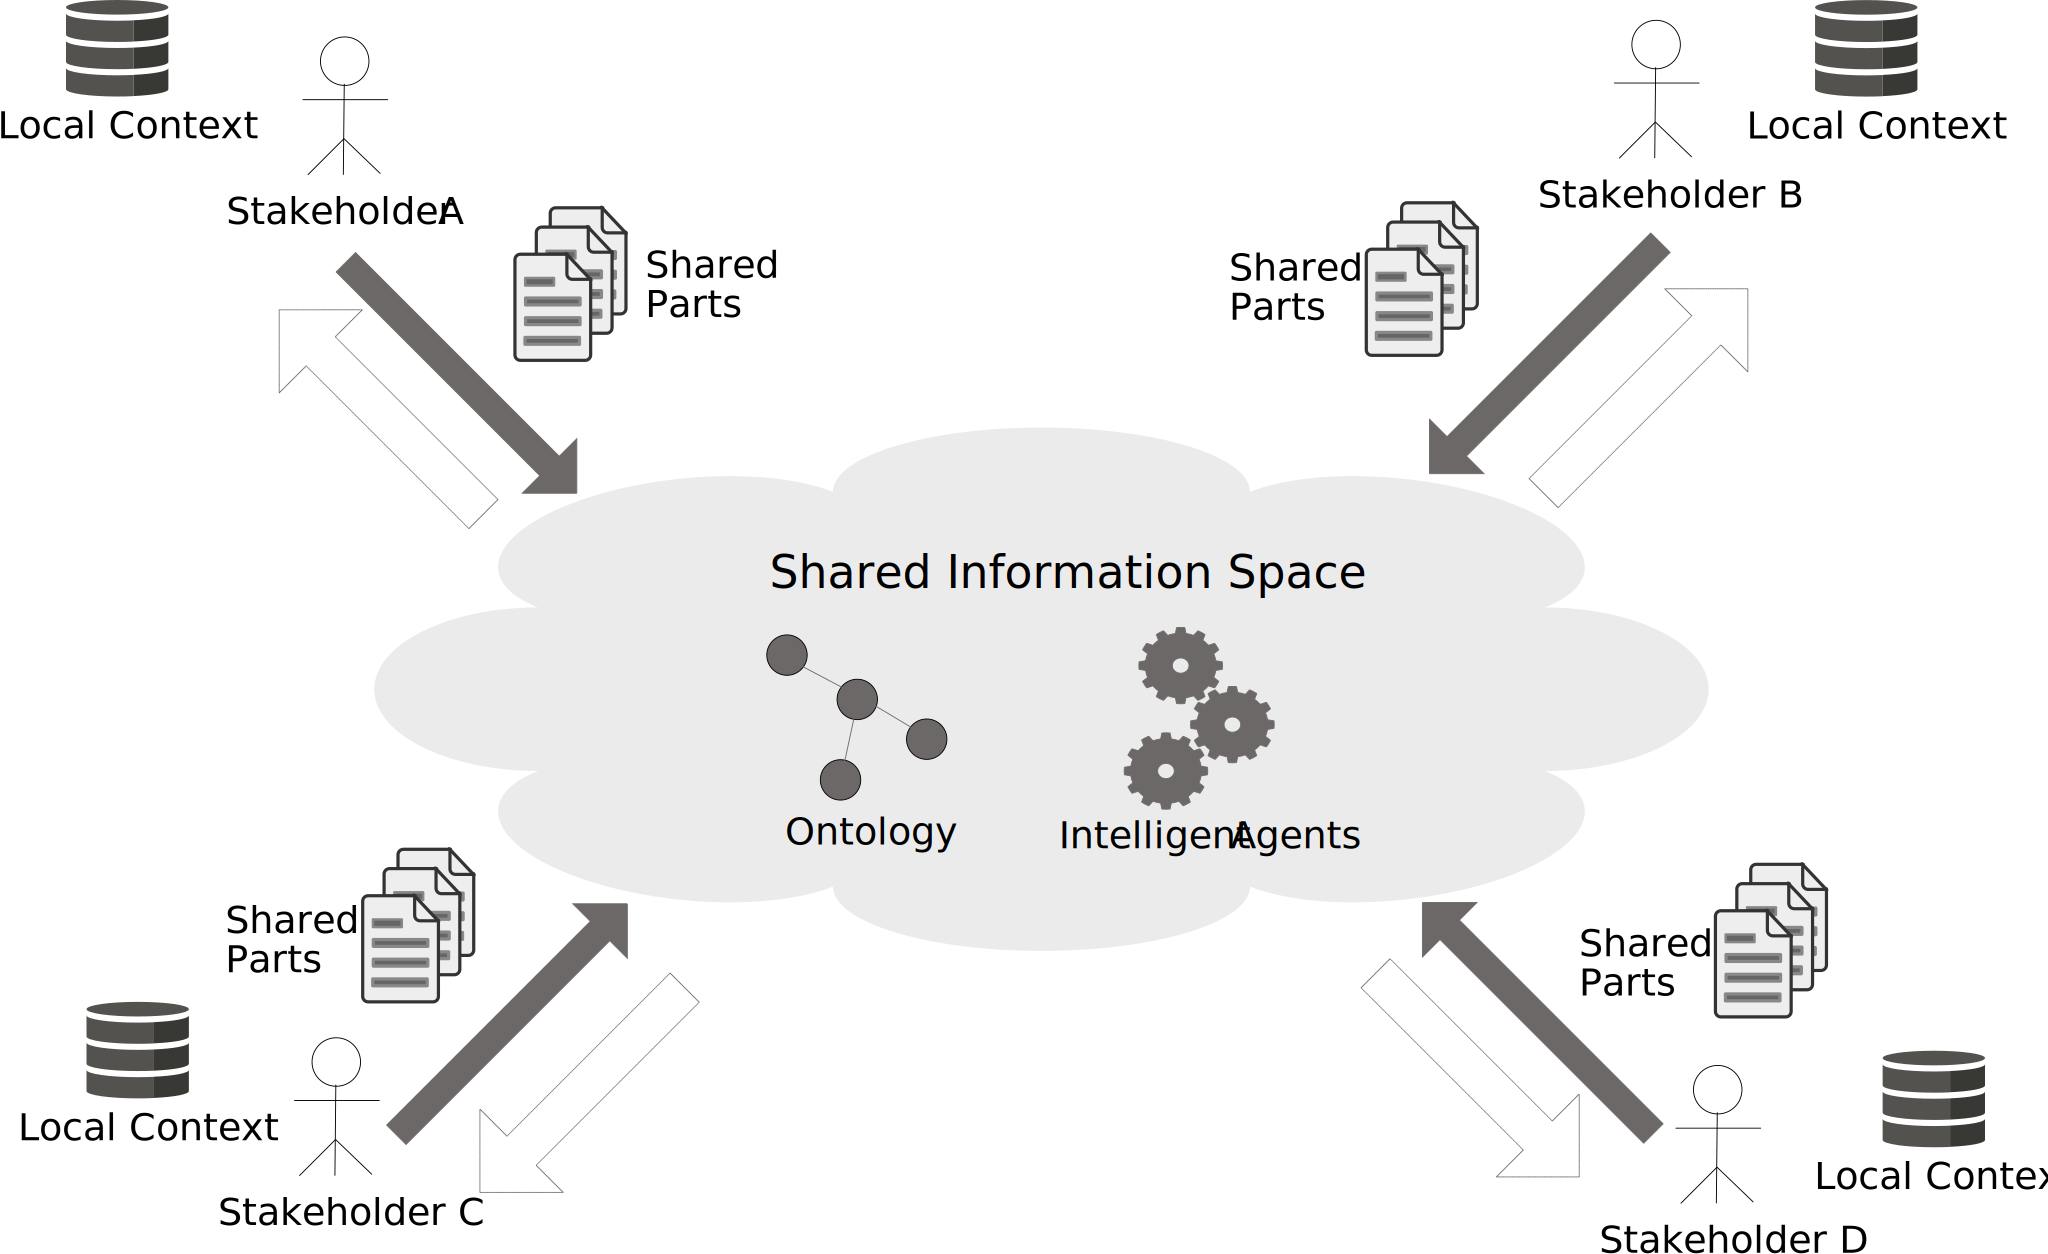
\includegraphics[width=0.9\columnwidth]{images/system_overview.pdf}
	\caption{System Overview}
\label{fig:images_system_overview}
\end{figure}

Due to the fact that data from various sources has to be combined into a shared understanding of the E-commerce activities of a consumer, there is the need to harmonize and transform the information into a shared data model. Based on the discussions in Chapter~\ref{cha:context_analysis} and the analysis of the information each stakeholder holds and transmits to others, the following initial information schema can be conducted (see Figure~\ref{fig:images_data_model}). This figure shows not only the relevant information from the local contexts of each stakeholder, but also how they can be combined within a shared information space. \\

\begin{figure}[!ht]
  \centering
  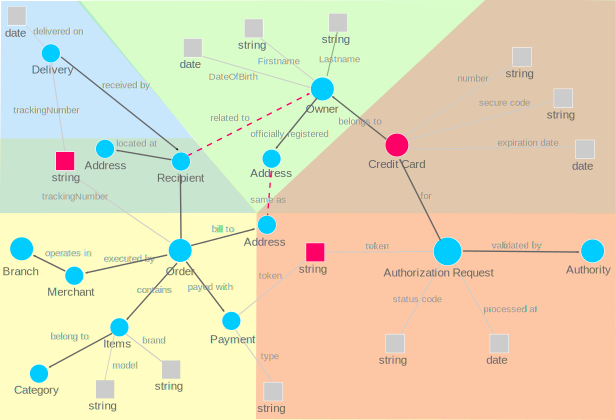
\includegraphics[width=0.9\columnwidth]{images/ontology_scenario_1.pdf}
  \caption{Data relations between stakeholders (green: Issuer, red: \gls{PSP}, yellow: Merchant, blue: \gls{LSP})}
\label{fig:images_data_model}
\end{figure}

As one can see there are connection points between these stakeholders. Those can be used as a reference for doing the merging of the information. There are actually three major connection points: \@

\begin{enumerate}
  \item \textbf{payment token}: shared between merchant and \gls{PSP}
  \item \textbf{tracking number}: shared between merchant and \gls{LSP}
  \item \textbf{credit card}: shared between issuer and \gls{PSP}
\end{enumerate}

In addition to these connection points one can also see the validation points in the Figure~\ref{fig:images_data_model}. These are critical points that have an influence on the decision whether an E-commerce transaction is suspecious or not. The criterias are: \@

\begin{enumerate}
  \item \textbf{billing address}: the billing address of the order has to match the registered address of the owner of the credit card used
  \item \textbf{recipient}: the recipient of the delivery has to be related to the owner of the credit card
\end{enumerate}

Whereas the first criteria can be examined during the authorization process of the credit card payment based on the information transmitted between merchant and \gls{PSP}, the second one is more difficult to validate (or can not be verified at all). The only check the \gls{LSP} is able to do before handing over the packaged items to the recipient, is to verify that she is the one mentioned in the order. If she is somehow related to the owner of the credit card or just a fraudster misusing the credit card data can not be confirmed at that point. \\

Also the merchant, the \gls{PSP} and the issuer are out of luck here. Whereas the merchant is able to validate whether the consumer has send items to that shipping address before, she can not restrict the consumer to choose only validated recipient addresses for shipping the order. Doing so will have a negative impact on the business of the online merchant. The \gls{PSP} and the issuer can not analyze this either, as both participants will not receive the information about the delivery address of the order in the credit card authorization request. \\

But just sharing the fact whether the shipping and billing address is different between the relevant stakeholders is not enough. Although this information is necessary, it is not sufficient to make a decision about suspecious transactions. Other necessary information are whether the consumer has send orders to this shipping address before, and the information about the content of the current order. Still, as mentioned in Section~\ref{sec:scope_thesis} looking at the single transaction of one merchant is not enough in the E-commerce fraud scenario that this thesis looks at. \\

Therefore the idea is to combine the transaction information from various merchants, \gls{LSP}s, \gls{PSP}s and issuers into one large, combined and shared information space to be able to analyze if there are any orders that look strange and are not being made by the owner of the credit card to a certain extend. One can already see that the proposed solution will have to deal with statistical evaluations and probabilities. \\

Starting with the credit card in question the issuer can query for the order details of transactions, that have been done recently with the credit card online. For that she might have to query the \gls{PSP} for the payment token first, before asking the merchant for order details to that payment token. At the end each online transaction can be mapped into a schema like the one shown in Figure~\ref{fig:images_data_model}, building up a large graph of entities and  the relationship between them, with the specific credit card in the center of it. An abbreviated sample graph of that can be seen in Figure~\ref{fig:images_credit_card_graph}. One can clearly recognize the different clusters of transactions by merchant. Still this first combination of the various order information into one data set is just the beginning of the analysis. Based on the information received the issuer can already filter out transactions, that have been shipped to different addresses than the credit card owner is registered for. Especially for those cases it might be worth to ask for additional information from the affected merchants to figure out if the consumer has used these shipping addresses before. As a result the existing graph can be enriched with additional transactional information from merchants at any time, if needed. In addition to the address information the issuer can also analyse the item information (incl.\ category, brand and model) of each order. \\

\begin{figure}[!ht]
  \centering
  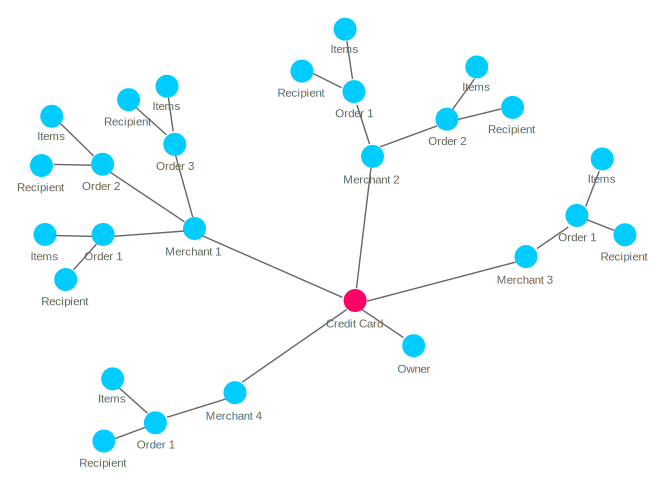
\includegraphics[width=0.9\columnwidth]{images/ontology_scenario_2.pdf}
  \caption{Clusters of E-commerce transactions by merchant}
\label{fig:images_credit_card_graph}
\end{figure}

But as shown in the Section~\ref{sec:scope_thesis} analysing the cluster of transactions from each merchant \textbf{\underline{alone}} will not be sufficient to come up with a solid decision about a suspecious transaction. This is due to the usage pattern of the fraudsters, that have been described in the scenario selected for this Master thesis --- using a credit card for ordering items from multiple merchants online. Therefore the various order details from the merchants have to be mapped against each other, so that the initial graph can be easily transformed into additional representations that uses different criterias to cluster the transactions --- such as recipient addresses, branches of the merchants, or product-related information. This reshaping of the graph can lead to new insights about the ``normal'' shopping behaviour of the credit card owner and make deviations from this behaviour visible. Visualizing the graph data as a clustered graph on screen supports the explorative nature of knowledge generation and perception, and can speed up the investigation of the E-commerce fraud incidents. An example visualization of a clustered graph is shown in Figure~\ref{fig:images_graph_viz}. \@

\begin{figure}[H]
  \centering
  \includegraphics[width=0.9\columnwidth]{images/GraphViz.png}
  \caption{An example visualization of a clustered graph \citep{visjsshowcase}}
\label{fig:images_graph_viz}
\end{figure}

 In addition to these graph visualizations the system can also support the investigation of the incidents by changing the type of visualization based on the criteria chosen for the clustering of the order details; e.g.\ when clustering them based on location information such as the shipping addresses the system can present the information as a heat map on a chart as displayed in Figure~\ref{fig:images_map_heatmap}. \@

\begin{figure}[H]
  \centering
  \includegraphics[width=0.9\columnwidth]{images/Heatmap.png}
  \caption{Heatmap displaying clusters of location-based information}
\label{fig:images_map_heatmap}
\end{figure}

% section system_overview (end)


% sub chapter existing approaches
%!TEX root = ../MasterThesis.tex

\section{Existing System Design Approaches}
\label{sec:system_approaches}

When trying to solve issues of information integration between organizations there are already existing solutions, that have to be examined whether they might fit the \gls{E-commerce} fraud investigation scenario or not.

\subsection{The \gls{ETL} processes}
\label{subsec:etl_process}

To begin with, retrieving, transforming and combining data from multiple dispersed data sources is not a completely new problem, and is actually part of ``Extract-Transform-Load'' or \gls{ETL} processes \emph{within} an organization. The basic idea is the same as in the concept shown in this thesis; namely to get as much information as possible from the various databases, that are in use within a company, harmonize (aka transform) the information from each of them into a shared data model, and use the cleaned up and combined information repository for doing advanced business analytics and predictions. Data within an organization is created and maintained by different business-related tools. Each of these will store the information into their own database using a vendor-specific schema. Other business-relevant data might be stored in structured files sometimes using a proprietary format, such as Excel files. Each of these data sources have to be accessed, the valuable information have to be extracted and mapped against each other, before the analysis of it can begin on a separate data store, that holds the combined data set. The whole process is visualized in Figure~\ref{fig:images_etl_process}. \\

\begin{figure}[!ht]
  \centering
  
\includegraphics[width=0.9\columnwidth]{images/etl_process.pdf}
  \caption[ETL process within a company]{\gls{ETL} process within a company \citep[pg. 165]{wood2014linked}}
\label{fig:images_etl_process}
\end{figure}

Still these \gls{ETL} processes rely on an in-depth knowledge of the data structures, that are used in each of the information sources as well as require a direct access to the databases and files for retrieving the information. Although these conditions are not cumbersome to work with within an organization, they will be a real show stopper if one has to integrate data sources across company boundaries. As the integration of the information takes place on the database level, allowing external access to your internal databases will not only open up access to your business internals, but will also make it much more complicated to change the underlying database structures and business-related software tools in use. Any changes to one of these require an elaborate negotiation between the owner of the data source and all of the external partners attached to it. \\

Beside this obviously unsuitable application for the \gls{E-commerce} fraud investigation scenario at the whole, one can assume that these \gls{ETL} processes are still in use for operating the daily business of each stakeholder. They can be helpful at a later point in the discussion, when a decision has to be made about how a stakeholder can prepare and transform his internal data sources for external consumptions.

% section etl_process

\subsection{Web Services}
\label{subsec:web_services}

With the development of the \gls{E-commerce} scenario there was also a need to integrate business functionalities from various service providers, whose are operating on the Internet. Valid examples for this kind of integration are the usage of the \gls{PSP} for doing the payment as well as the \gls{LSP} for handling the shipping process. These approaches resulted in the ``Service Oriented Architecture'' paradigm, that enables application services provided by different vendors to talk to each other via a public facing programming interface (aka \gls{API}). The only requirement for such interoperability to work properly is, that each public interface follows some standardized or commonly agreed upon guidelines to be vendor-, platform- as well as language-agnostic. One possible implementation of these concepts are the so-called Web Services, that use the WS* protocols and standards from the \gls{W3C} with the extensible markup language (aka \gls{XML}) and the \gls{HTTP} protocol at their core \citep{josuttis2007soa}. \\

Like the \gls{HTML} format, that is used to represent Web pages on the Internet, \gls{XML} is originally based on \gls{SGML}, but instead of formalizing markup tags for structuring and styling textual content it is a meta-language allowing everyone to define his or her own markup languages. In this matter it doesn’t dictate what tags are available to structure the information; instead it includes some basic guidelines for creating well-formed and valid documents that uses domain-specific tags, which can be freely defined and structured by the creator of the \gls{XML} document. Therefore it is better suited in situations, in which a computer has to parse and evaluate the content of a message; assuming the computer program knows the structure of the message. \\

In an additional step the author of the \gls{API} could also specify an \gls{XML} schema for each message, which describes the structure of the message with all the possible elements, their ordering, nesting level and data types in detail. By doing so the \gls{XML} parser program can later verify the content of a retrieved message against the \gls{XML} schema and check if it is a valid document related to the schema definition. \gls{XML} schemata are also expressed in \gls{XML} format and have been standardized by the \gls{W3C}. Being able to create custom markup languages via \gls{XML} has a huge benefit for machine-to-machine communication and is the basis for integrating Web Services (via the WS* protocols), but it still has limitations when it comes to figure out the semantics of those \gls{XML} messages. This is mostly due to the fact that each \gls{XML} document represents a new markup language and needs a specific \gls{XML} parser to be understood by the machine; also to distinguish commonly used tag names in an \gls{XML} document the creator has to place them into specific namespaces (aka \gls{XML} namespaces). But those \gls{XML} namespaces further complicate the automatic processing of \gls{XML} documents and increases the necessity to have custom instances of \gls{XML} parsers for each \gls{XML} document \citep{taylor2008p2p}. \\

An integration of information exchange via Web Services is usually handled separately for each Web Service interface. Looking at the payment service integration as \emph{one} possible example, the following steps are necessary to allow a merchant to interact with the Web Service of a \gls{PSP}: \@

\begin{itemize}
  \item the \gls{PSP} has to define and implement an interface (aka \gls{API}) that a merchant can use to exchange information with them
  \item the \gls{API} includes a set of data exchange messages, usually in \gls{XML} format, as well as a list of operations, that the interface supports
  \item the \gls{PSP} has to document each of these messages and operations, incl.\ their intended structures and semantics
  \item the \gls{PSP} has to provide access to the \gls{API} via an \gls{HTTP} endpoint running on a server at a specific \gls{URL}
  \item the \gls{PSP} usually restricts access to this interface for registered partners only; for this they have to provide a registration and identification mechanism
  \item the merchant has to register with the \gls{PSP} to be able to call into their Web Service \gls{API}
  \item the merchant receives some kind of token, that they can use to identify themselves with the Web Service later
  \item the merchant has to implement an \gls{API}-specific client-side wrapper, that knows how to talk to the interface; incl.\ calling one of the available operations as well as serializing and deserializing the messages that will be transmitted between the Web Service and the client program
  \item the client program has to understand the structure and semantic of the messages exchanged with the Web Service
\end{itemize}

Although other merchants, that want to use the same \gls{API} from the \gls{PSP}, can use the same client-side wrapper (sometimes also provided by the \gls{PSP} for convenience) to send/receive messages to/from this specific Web Service, they still have to make the \gls{API}-specific integration into their own Web shop. Also, the integration is only done in an one-way direction. To allow the merchant to provide information from their own databases, the merchant has to do likewise and provide an \gls{API} for others to use to query for information (following the same steps as mentioned above). \\

Also, as the structures and semantics of the messages and operations of each Web Service interface are not standardized, integrating with another \gls{PSP} or merchant results in doing the same integration steps again and again. To make things worse, the mapping of the information coming from different \gls{API}s has to be implemented by the client, who wants to analyze the combined data set.   It soon becomes clear, that these necessary tasks will increase the time and effort with each additional stakeholder, who wants to participate in the collaborative system, see Figure~\ref{fig:web_services_scenario}. \@

\begin{figure}[H]
  \centering
  \includegraphics[width=0.9\columnwidth]{images/web-services-scenario.pdf}
  \caption{The Web Services scenario}
\label{fig:web_services_scenario}
\end{figure}

As conclusion one could easily see that integrating information between a larger group of participants is very limited with the existing Web Services approach. The steps necessary for exchanging information result in huge efforts on all participating parties. As there is no common way to access and combine the information from each one of the participants, beside using the fundamental \gls{HTTP} protocol and \gls{XML} data format, there have to be a lot of collaborative work between each of them upfront, to come up with an approach to integrate the available \gls{API}s, and provide the rules for combining the different data structures. Due to these restrictions one can assume that an integration based on the Web Services approach will only work with a limited number of participants. This might lead to a collaborative system, that will only include larger online retailers as participants, and therefore left out smaller shops from the \gls{E-commerce} fraud investigation process. For a solution of the problem described in Section~\ref{sec:scope_thesis} this is not sufficient. One need technologies that provide a better scalability and integration ability for the exchange of information between various, otherwise not strongly related organizations.

% subsection web_services (end)

\subsection{Semantic Web}
\label{subsec:web_data}

``The Web is full of intelligent applications, with new innovations coming every day'' \citep{allemang2011semantic}. But each of those intelligent Web applications is driven by the data available to them. Data that is likely coming from different places in the global information space — accessible usually via a custom API on the server hosting those resources (see Section~\ref{subsec:web_services}). The more consistent the data available to the smart Web application is, the better the Web service and its result will be. But to support an integration of the data from various Web services the semantics of the information delivered by each service has to be available — and there has to be a generalized, formalized way to express the semantic of that data. The focus on a standard that allows Web services to express the semantics of the data they provide also allows for global scalability, openness and decentralization, which are the key principles of the World-Wide Web. The Semantic Web tries to give a solution for this problem by providing the Resource Description Framework (aka \gls{RDF}) and related technologies (e.g. RDF schema, \gls{SPARQL}, \gls{OWL}, \ldots) for describing, linking and querying the data that a Web service delivers. But it doesn’t reinvent the wheel; instead the Semantic Web builds upon existing, proven technologies like \gls{XML}, XML namespaces, XML schemata and the \gls{URI} to uniquely address resources on the Web \citep{allemang2011semantic}. \\

The main benefits of the Semantic Web approach are the specification of a standardized and generalized format to exchange information on the Web (aka \gls{RDF}) as well as a commonly agreed way to access and query for them (aka \gls{SPARQL}). The \gls{RDF} data format does not only specify the syntax of the information exchanged, but also include the semantic (aka meaning) of them. Due to this fact, resources described in \gls{RDF} format are consistent and semantically self-contained. These characteristics are achieved by providing information as a ``triple''; that is a statement consisting of the resource in question (aka subject), a predicate and the specific value (aka object) for it. To be able to unambiguously identify the meaning of these statements, each part of them are usually expressed by utilizing unique \gls{URI}s. These \gls{URI}s can be abbreviated via ``prefix'' definitions to make the whole statement easier to read (see also Section~\ref{sec:semantic_web}). To specify that there is an order ``12345'' from ``merchant1'', one can come up with the following statement, that uses the explicit Schema.org specification \citep{Schema.org} to describe an order: \@

\begin{listing}[H]
  \inputminted[linenos,
               numbersep=5pt,
               breaklines=true,
               frame=lines]{TURTLE}
               {./samples/sample_order_12345.ttl}
  \caption{An order specification in \gls{RDF}}
\label{lst:sample_order_ttl}
\end{listing}

An \gls{RDF} file can contain one or more of such ``triples'' describing the resources of interest in detail. Usually these ``triples'' are visualized as directed graph, in that subjects and objects are displayed as nodes and predicates as edges between them. The above Listing~\ref{lst:sample_order_ttl} can be presented as graph like this:\@

\begin{figure}[H]
  \centering
  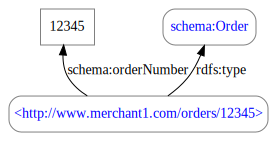
\includegraphics[width=0.8\columnwidth]{images/sample_order_12345.pdf}
  \caption{Graph-based visualization of \gls{RDF} from Listing~\ref{lst:sample_order_ttl}}
\label{fig:sample_order_graph_image}
\end{figure}

Beside having to provide internal resources in an understandable \gls{RDF} format the Semantic Web also specifies how to query and access the ``information databases'' on the Web. For this purpose the \gls{SPARQL} language and protocol is used. It does not only describe a query language, but also shows how to setup an \gls{HTTP} endpoint on a server to make the data set publicly available on the Internet. \\

Based on the specifications of the Semantic Web standards each relevant participant of an \gls{E-commerce} fraud investigation system will have to transform the information from their internal databases into a set of ``triples'' with commonly agreed upon \gls{URI} references. These additional data sets will be made available publicly on the Web for information retrieval via the \gls{SPARQL} language and protocol. Each participant of the collaborative system just needs to know the specific addresses of the \gls{SPARQL} endpoints to be able to query them for information. The results of each query can be easily combined into a new data set based on the merging capabilities of the \gls{RDF} standard. This will decrease the efforts for integrating the data from various external sources drastically. Also communicating with the different \gls{HTTP} endpoints to access and query for information is being done in a much more efficient way based on the \gls{SPARQL} protocol, see Figure~\ref{fig:web_data_scenario}. \@

\begin{figure}[H]
  \centering
  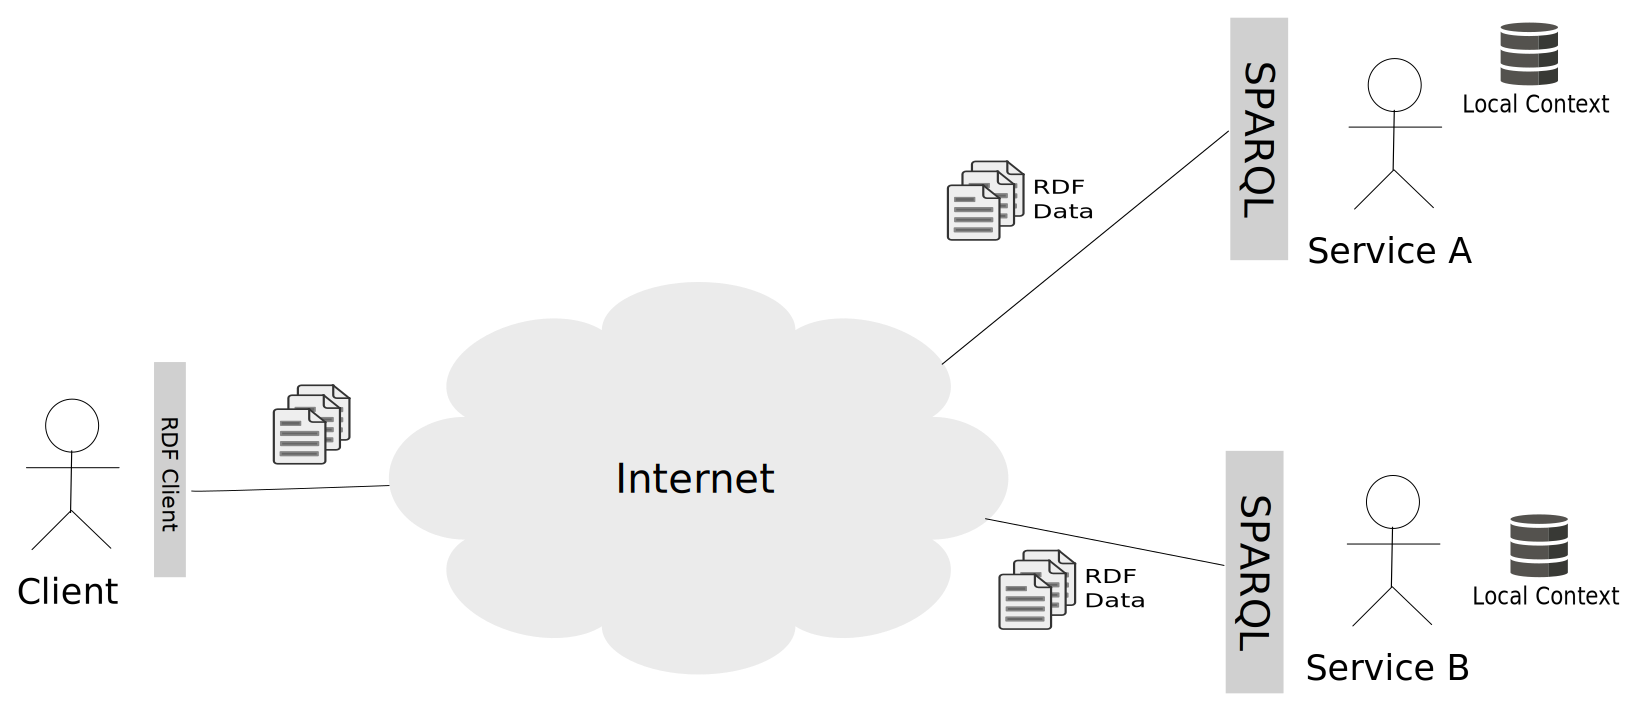
\includegraphics[width=0.9\columnwidth]{images/web-data-scenario.pdf}
  \caption{The Semantic Web scenario}
\label{fig:web_data_scenario}
\end{figure}

As the underlying model of an \gls{RDF} data set is resembling a graph-based representation it will fit the concept of the proposed system from Section~\ref{sec:design_proposal} perfectly. Still requiring any participant to setup and operate a public available \gls{SPARQL} server will limit the use of this architecture for the solution of the \gls{E-commerce} fraud investigation scenario. As parts of the information, that have to be exchanged between the relevant participants are confidential and/or business-critical to them, requiring a public \gls{HTTP} endpoint on the Internet, is a high security risk. Additionally the \gls{SPARQL} language and protocol does not offer a way to restrict access to only a subset of the information in the \gls{RDF} data store. Any party, who is aware of the \gls{URL} of the \gls{SPARQL} endpoint have access to all the information, that are in the underlying \gls{RDF} data stores (see Listing~\ref{lst:get_them_all_sparql}). It is therefore no surprise, that there are currently only a small set of publicly available \gls{SPARQL} endpoints on the Internet --- with the most commonly used one from DBpedia.org \citep{dbPedia.org}, that is offering public available data from Wikipedia articles in \gls{RDF} format. \@

\begin{listing}[!ht]
  \inputminted[linenos,
               numbersep=5pt,
               breaklines=true,
               frame=lines]{SPARQL}
               {./samples/get_all_records.sparql}
  \caption{Retrieving all information in an \gls{RDF} store using \gls{SPARQL}}
\label{lst:get_them_all_sparql}
\end{listing}

To conclude, one can assert that the fundamental technologies of the Semantic Web standards are a good fit for exchanging and merging information between different stakeholders. But the usage of an all or nothing approach for querying the \gls{RDF} data stores via \gls{SPARQL} is way to open for the proposed solution.

% subsection web_data (end)

% section system_approaches (end)


% sub chapter design proposal
%!TEX root = ../MasterThesis.tex

\section{System Design Proposal}
\label{sec:design_proposal}

As the previous section showed, existing approaches are of limited use for the design of a collaborative system to support the \gls{E-commerce} fraud investigation scenario described in Section~\ref{sec:scope_thesis}. The leading approach for such a system will have to combine the best characteristics from the Web Service and the Semantic Web designs. \\

As for the Web Service approach, the most valuable aspects of it are: \@

\begin{itemize}
	\item access to the \gls{HTTP} endpoints can be limited to a certain set of communication partners
	\item these partners have to authenticate with each Web Service first
	\item based on the identification of the partners only certain parts of information can be returned, and execution of operations can be restricted
\end{itemize}

Looking at the Semantic Web approach, it's most interesting functionalities are: \@

\begin{itemize}
	\item providing information in a semantically self-contained way
	\item the ability to merge information from different \gls{RDF} data stores
	\item the graph-based data model underlying the \gls{RDF} data stores
	\item the usage of \gls{SPARQL} to query and analyze the locally combined data sets
\end{itemize}

In the following section the thesis will come up with an approach that uses the fundamental technologies from the Semantic Web for information sharing and integration as well as peer-to-peer communication technologies for securing and restricting access to the \gls{RDF} data sets from the relevant participants of the \gls{E-commerce} fraud investigation scenario. It will start with a discussion of the semantics of the underlying \gls{RDF} files and how these can be combined across various organizations. After that it shows how these information can be provided to the relevant parties in the investigation scenario. It will continue with a detailed look into the partially centralized \gls{P2P} communication architecture and how that can be used for the proposed solution.

\subsection{Vocabulary alignment}
\label{subsec:vocab_align}

Although the \gls{RDF} format has build-in support for merging information from different data sources, this functionality is only working as expected if the ``triples'' in the dispersed data stores are using the same \gls{URI}s to refer to the same subjects or objects. In that case merging the ``triples'' from different \gls{RDF} data files will result in a local graph holding the combined information as shown in Figure~\ref{fig:images_combine_rdf_graph}. \\

\begin{figure}[!ht]
	\centering
		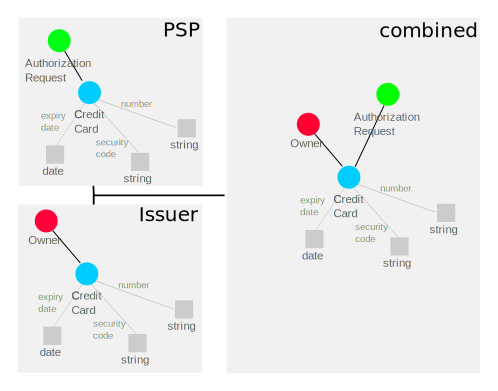
\includegraphics[width=0.9\columnwidth]{images/combine_rdf_graph.pdf}
	\caption{Combining two \gls{RDF} files containing the same credit card entity}
\label{fig:images_combine_rdf_graph}
\end{figure}

As a major objective of the \gls{E-commerce} fraud investigation system is to bring the various transactional information from online merchants, \gls{PSP}s and issuers together, combine them all and analyze the resulting graph from different viewpoints, the information exchanged between the relevant participants have to follow a common schema. A possible approach is to define a completely new schema for the proposed system and share it with every possible stakeholder. This schema will define all the entities and relations known to the collaborative system and would be expressed in \gls{RDFS} format. A major drawback of this approach is, that new partners of the system will have to do the conversion of their internal data structures to an \gls{RDF} file, that is compatible with the specific schema definition, before being able to participate in it. \\

Therefore a better approach is to take a look into commonly used \gls{RDF} schemata and vocabularies, and try to figure out if they can be used for describing the information, that need to be exchanged between participants of the \gls{E-commerce} fraud investigation system. When consulting the Semantic Web community for commonly agreed upon and highly referenced \gls{RDF} schema definitions, one will come up with this list (see Table~\ref{tab:used_vocab_rdf}):\@

\begin{table}[H]
\centering
\begin{tabular}{p{3cm}llp{4.5cm}}
\hline
\textbf{Name} & \textbf{Prefix} & \textbf{Describes} & \textbf{Namespace URI} \\
\hline
Dublin Core & dc: & Meta data & \url{http://purl.org/dc/terms/} \\
\hline
FOAF & foaf: & People & \url{http://xmlns.com/foaf/0.1/} \\
\hline
Geo & pos: & Positions & \url{http://www.w3.org/2003/01/geo/wgs84\_pos\#} \\
\hline
Geo Names & gn: & Locations & \url{http://www.geonames.org/ontology\#} \\
\hline
Good Relations & gr: & Products & \url{http://purl.org/goodrelations/v1\#} \\
\hline
RDF & rdf: & Core framework & \url{http://www.w3.org/1999/02/22-rdf-syntax-ns\#} \\
\hline
RDFS & rdfs: & RDF vocabularies & \url{http://www.w3.org/2000/01/rdf-schema\#} \\
\hline
Schema.org & schema: & Schema.org vocabularies & \url{http://schema.org/} \\
\hline
SKOS & skos: & Controlled vocabularies & \url{http://www.w3.org/2004/02/skos/core\#} \\
\hline
vCard & vcard: & Business Cards & \url{http://www.w3.org/2006/vcard/ns\#} \\
\hline
Web Ontology Language & owl: & Ontologies & \url{http://www.w3.org/2002/07/owl\#} \\
\hline
XML Schema Datatypes & xsd: & Data types & \url{http://www.w3.org/2001/XMLSchema\#} \\
\hline
\end{tabular}
\caption[Commonly used \gls{RDF} vocabularies on the Web]{Commonly used \gls{RDF} vocabularies on the Web \citep[pg. 41]{wood2014linked}}
\label{tab:used_vocab_rdf}
\end{table}

Based on these schema specifications describing a fictive consumer named ``Max Mustermann'' incl.\ his home address can be done by combining data utilizing the \gls{FOAF} and \gls{vCard} namespaces in a \gls{RDF} file, such as described in Listing~\ref{lst:sample_customer_mustermann} and visualized as graph in Figure~\ref{fig:images_sample_customer}. \@

\begin{listing}[H]
  \inputminted[linenos,
               numbersep=5pt,
               breaklines=true,
               frame=lines]{TURTLE}
               {./samples/sample_customer_mustermann.ttl}
  \caption{Personal related information about a fictive consumer in \gls{RDF}}
\label{lst:sample_customer_mustermann}
\end{listing}

\begin{figure}[H]
	\centering
		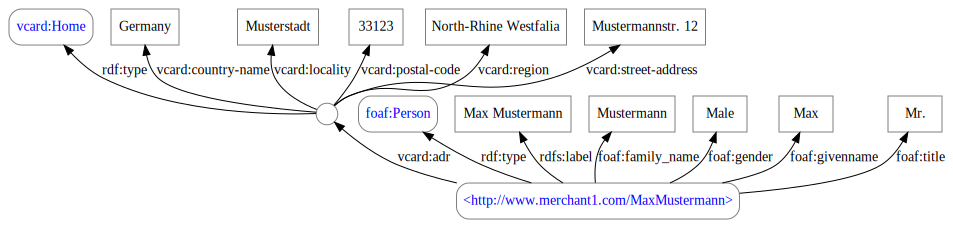
\includegraphics[width=\columnwidth]{images/sample_customer_mustermann.pdf}
	\caption{Graph representation of consumer information from Listing~\ref{lst:sample_customer_mustermann}}
\label{fig:images_sample_customer}
\end{figure}

Looking back to the initial data model from Section~\ref{sec:system_concept} one can map the information, that are currently available in the \gls{E-commerce} scenario, to the existing \gls{RDF} vocabularies such as follows (see Table~\ref{tab:map_tx_rdf_vocab}):\@

\begin{table}[H]
\centering
\begin{tabular}{p{5cm}l}
\hline
\textbf{Information} & \textbf{RDF vocabulary} \\
\hline
Consumer & FOAF \\
\hline
Credit Card Owner & FOAF \\
\hline
Billing Address & vCard \\
\hline
Shipping Address & vCard \\
\hline
Location Information & Geo Names \\
\hline
Merchant & GoodRelations \\
\hline
Items & GoodRelations \\
\hline
Item Categories & GoodRelations \\
\hline
Brands & GoodRelations \\
\hline
Payment Types & GoodRelations \\
\hline
\end{tabular}
\caption{Possible usage of \gls{RDF} vocabularies for \gls{E-commerce} transaction information}
\label{tab:map_tx_rdf_vocab}
\end{table}

As this table shows there are some parts of the \gls{E-commerce} data model that can be expressed with existing \gls{RDF} vocabularies extensively --- such as personal related information via \gls{FOAF} and \gls{vCard}, whereas other parts can not be stated in-depth (e.g. credit card information), or are not specified at all (e.g.\ tracking of the delivery). Additionally some of the vocabularies are no longer actively maintained, such as GoodRelations. Due to these circumstances one usually have to build an own ontology that fills in the missing pieces and refers to the existing concepts whenever appropriate. Trying to model the information of a credit card as displayed in Figure~\ref{fig:images_data_model} will result in the \gls{RDFS} specification shown in Listing~\ref{lst:credit_card_vocab}. \@

\begin{listing}[H]
  \inputminted[linenos,
               numbersep=5pt,
               breaklines=true,
               frame=lines]{TURTLE}
               {./samples/vocab_credit_card.ttl}
  \caption{A specification for a credit card in \gls{RDFS}}
\label{lst:credit_card_vocab}
\end{listing}

But building a new ontology for handling the \gls{E-commerce} fraud investigation process is not the best approach. The result would be that participants have to access, understand and implement the desired \gls{RDF} data schema first, before they can share their information in the collaborative system. Looking back at the list of existing ontologies and vocabularies, that are actively used on the Web today, one will find the Schema.org vocabulary definition \citep{Schema.org}. This vocabulary was initially designed by the leading search engines (aka Google, Microsoft and Yahoo!) to allow authors of Web sites to markup their \gls{HTML} documents in a way, that they are better understood by those search engines (aka \gls{SEO}). The Schema.org vocabulary is actively maintained by its community, includes new concepts with each release and also offers an extension mechanism to implement additional vocabularies that are not part of the core specification \citep{SchemaExtensions}. In one of the past releases of the Schema.org core specification it also included all of the existing concepts of the GoodRelation ontology \citep{SchemaGoodRelation}. \\

As the merchants will provide semantic meta data for their products to improve their listing on search engine results (aka \gls{SEO}) in the vocabulary of Schema.org already, one can re-use parts of these information for the \gls{E-commerce} fraud investigation. Additionally, the wide-ranging scope of aspects that Schema.org declares make it a good fit to the \gls{E-commerce} fraud investigation scenario. Trying to map the initial data model from Section~\ref{sec:system_concept} to the Schema.org core specification will result in a data schema as displayed in Figure~\ref{fig:images_schema_org}. \@

\begin{figure}[!ht]
	\centering
		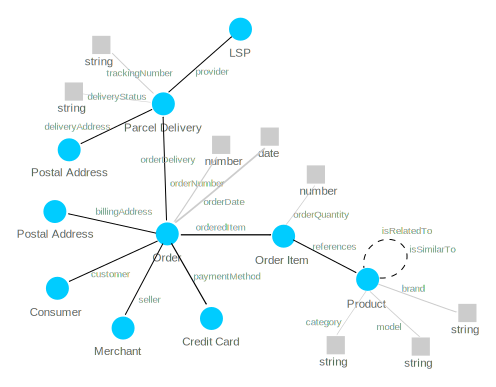
\includegraphics[width=0.8\columnwidth]{images/schema_org_mapping.pdf}
	\caption{Schema.org based mapping of an \gls{E-commerce} transaction}
\label{fig:images_schema_org}
\end{figure}

% subsec vocab_align

\subsection{Communication protocols}
\label{subsec:comm_protocol}

 The data is likely encoded in Microdata, \gls{RDFa} or \gls{JSON-LD}. \\

For the communication the \gls{WebRTC} is a good approach as it integrates well with existing enterprise IT infrastructures.
\\

\ldots

% subsec comm_protocol

\subsection{Using a partially centralized \gls{P2P} system}
\label{subsec:p2p_partially_centralized_system}

For the \gls{E-commerce} fraud scenario, that has been selected for this thesis in Section~\ref{sec:thesis_scope}, one can say that the issuer of a credit card is the party who initiates the collaborative fraud investigation. They are recognizing the active use (and likely misuse) of a credit card in the online and the offline world first, and are also getting a notification about any suspicious transactions made with it from their fraud prevention systems. Due to this fact, one can come up with a partially centralized \gls{P2P} architecture for the \gls{E-commerce} fraud investigation system, in that the issuer of a card in at the center and acts as a trusted party in this system. This issuer will initiate a collaborative session with the other required stakeholders based on the usage history of the credit card in question. During this \gls{P2P} communication session the merchants, \gls{PSP}s and \gls{LSP}s will share the required information with the issuer. In this process the data from the other stakeholders will be replicated to the issuer, who will build up a networked graph based on the Schema.org specification. So the main work will be on the issuer's side, who is the major driving party in the system, as depicted in Figure~\ref{fig:images_p2p_centralized}.\@

\begin{figure}[H]
	\centering
		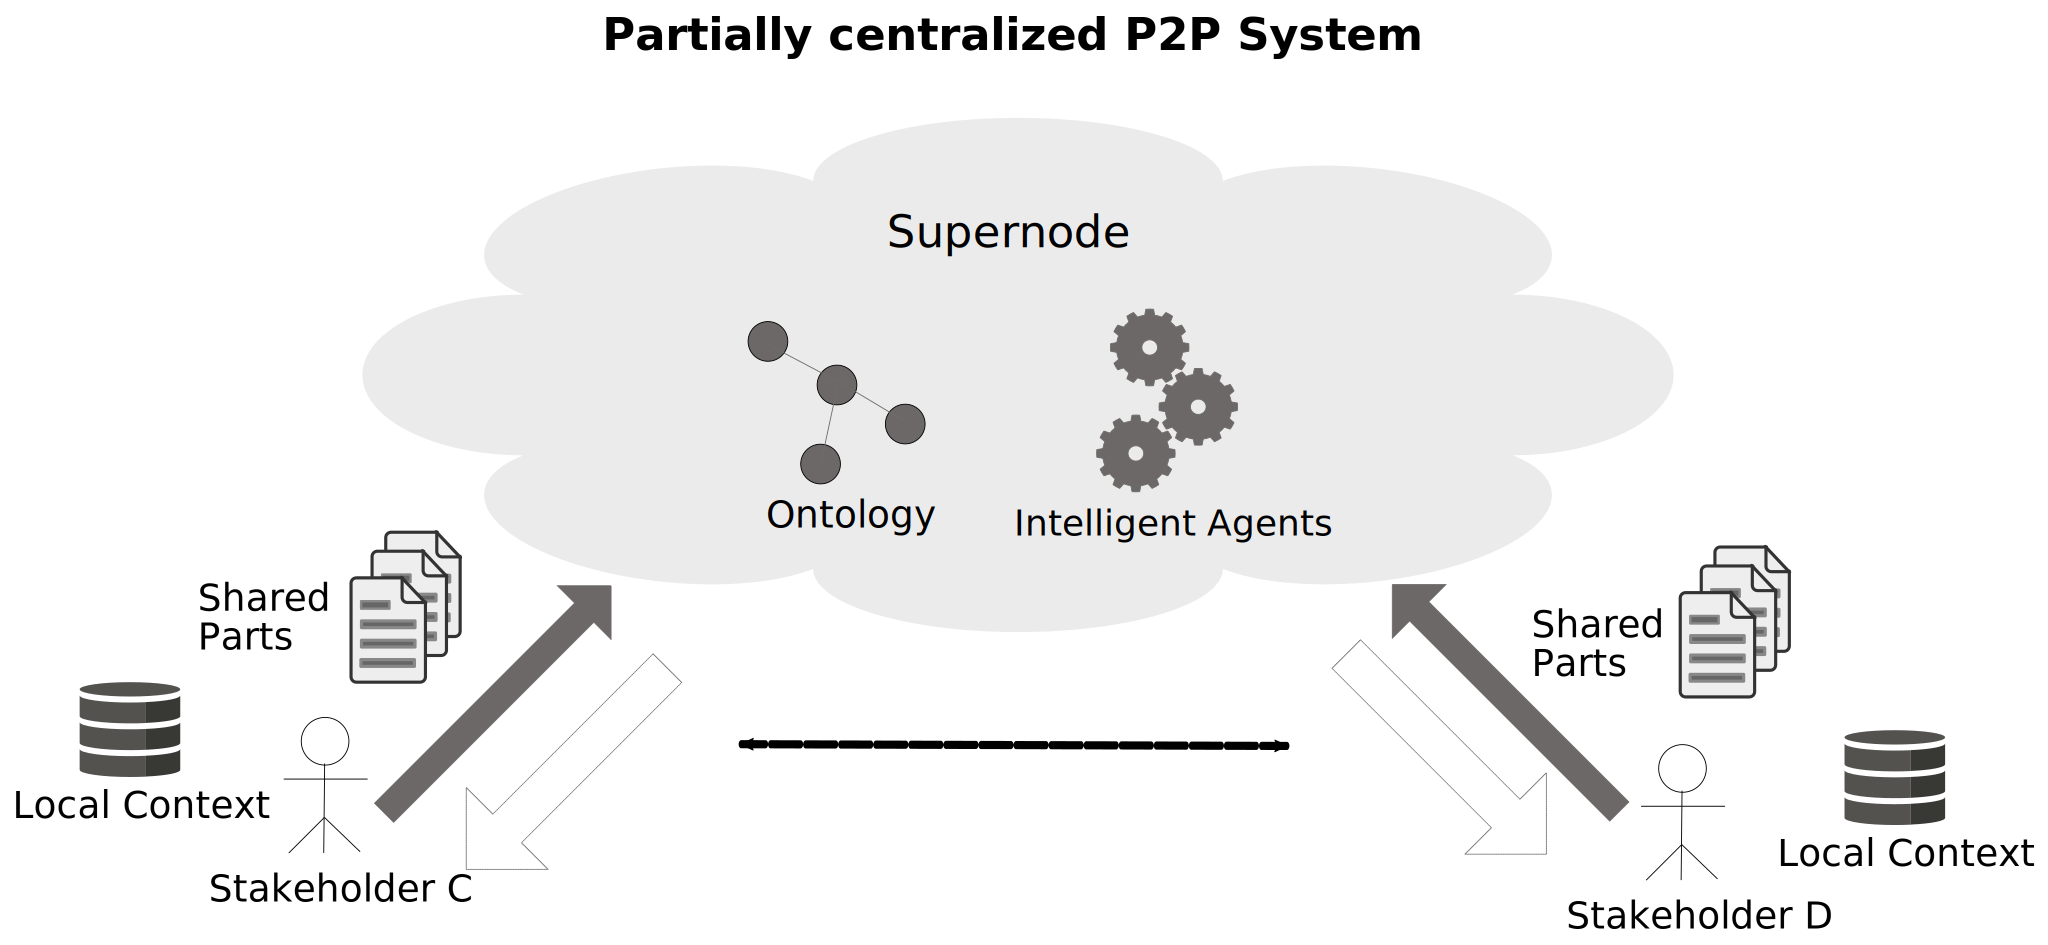
\includegraphics[width=0.9\columnwidth]{images/system_P2P_centralized.pdf}
	\caption{Collaborative system using a partially centralized \gls{P2P} architecture}
\label{fig:images_p2p_centralized}
\end{figure}

Using the \gls{WebRTC} communication protocol for initiating the \gls{P2P} session will allow the issuers to setup a communication between the relevant stakeholders directly from within an application running in their Web browsers. The application can visualize the connectivity status of the participants, the progress of their data sharing efforts as well as offer direct face-to-face communication possibilities in case of misunderstandings or further requests. A wireframe of the Web application screen is depicted in Figure~\ref{fig:images_p2p_initial_screen}. \@

\begin{figure}[H]
	\centering
		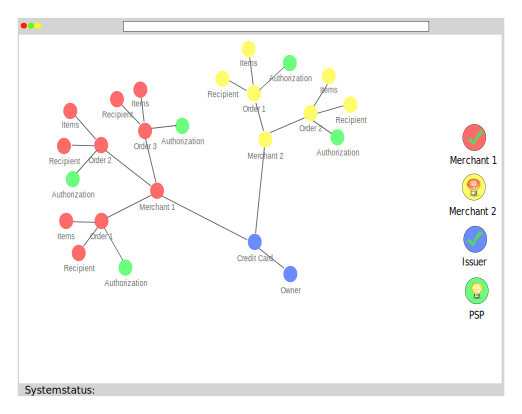
\includegraphics[width=0.9\columnwidth]{images/p2p_initial_screen.pdf}
	\caption{Screen prototype of collaborative system showing participants and shared information}
\label{fig:images_p2p_initial_screen}
\end{figure}

One of the major issues with the above mentioned system architecture is, that the merchants, \gls{PSP}s and \gls{LSP}s have to hand over all of their relevant information to the issuer of a credit card for the analysis. \\

\ldots

% subsec p2p_partially_centralized_system

% section design_proposal (end)


% chapter design system (end)
